\documentclass[11pt]{article}
\usepackage[margin=1in]{geometry}
\usepackage{amsmath,amssymb,amsthm}
\usepackage{booktabs,longtable}
\usepackage{tikz}
\usepackage[hidelinks]{hyperref}

\newtheorem{theorem}{Theorem}
\newtheorem{lemma}[theorem]{Lemma}

\newcommand{\lean}[1]{{\small\texttt{#1}}}
\newcommand{\RN}{\mathrm{RN}}

\title{How far FRECPE's reciprocal can drift in \texttt{logf}:\\
a machine-checked bound}
\author{}
\date{}

\begin{document}
\maketitle

\begin{abstract}
A \texttt{logf} built on the Arm instruction FRECPE takes its reciprocal from an
8-bit estimate instead of a table, and stays within one ulp of the correctly
rounded result over every binary32 input. This note proves how much further that
reciprocal could drift and keep that guarantee: for each of FRECPE's 256 cells,
a window of reciprocals within which every input is within one ulp. Away from
$x = 1$ the windows reach about $\pm 4\%$, against FRECPE's own error of at most
$0.29\%$ over a cell. The proof is checked by Lean~4 with Mathlib; each statement below names
its Lean counterpart in \lean{proof/lean/FrecpeLogf/}. It is the \emph{bound-only}
proof: one analytic bound per cell. Section~\ref{sec:exact} says how it extends to
an exact one.
\end{abstract}

\section{The result}

Write $x = 2^k m$ with $m \in [1, 2)$ and let \emph{cell} $i$ hold the significands
whose top eight fraction bits are $i$. FRECPE returns the same estimate
$\hat c(i)$ for the whole cell. The kernel uses $c_i = \hat c(i)$, except
$c_0 = 1$: FRECPE's $511/512$ breaks one ulp just above $x = 1$. It then computes
$r = m c - 1$ and $\log x \approx k \ln 2 - \log c + P(r)$, where $P$ is glibc 2.44's
polynomial and $-\log c$ comes from a table.

\begin{theorem}[\lean{frecpe\_logf\_drift\_bound}]\label{thm:main}
For each cell $i$ there are rationals $\varepsilon^-_i, \varepsilon^+_i \ge 0$,
listed in Appendix~\ref{app:table}, such that for every real $m$ with
$1 + \tfrac{i}{256} \le m \le 1 + \tfrac{i+1}{256} - 2^{-23}$ (the significands of cell $i$),
every exponent $k \in [-149, 127]$ with $m \ge 1 + 2^{-23}$ when $k = 0$ (so $x \ne 1$),
and every real
$c \in [c_i(1 - \varepsilon^-_i),\ c_i(1 + \varepsilon^+_i)]$: the kernel run with $c$
and with the log entry rounded for $c$ returns $\RN_{32}(\log x)$ or a binary32
adjacent to it.
\end{theorem}

The theorem holds for every real $c$ in the window, not only those on a particular
grid, so it covers any reciprocal representable in binary64.

The windows are close to what the kernel actually tolerates. Across the 512 sides
(256 cells, each way), compared with the search over every input in
\lean{table-tolerance.cpp}, section B4:

\begin{itemize}
\item the proven bound is never more than a factor $1 + \tfrac{3}{256}$ past the measured one
(\lean{gen/check.py} fails otherwise), and all but 5 sides are within 2\% of it;
\item the median tighter side is $3.875\%$, and over cells 2 to 253 it runs from
$2.43\%$ to $4.48\%$;
\item in cell 68 upward, where every $c$ on the 29-bit grid around the bound was
scanned, the proven $3.8706\%$ sits just under the exact edge of $3.87458\%$;
\item in a run of the compiled kernel on an M5 (\lean{make proof-hw}), at $\tfrac14$, $\tfrac12$,
$\tfrac34$ and all of each side's proven drift against every input of the cell (2048
points, $1.7 \times 10^{10}$ evaluations), no input passed one ulp.
\end{itemize}

\section{The floating-point model}\label{sec:model}

Nothing is assumed of the hardware beyond the hypotheses below; they are hypotheses of
the theorem, not axioms of the development.

\paragraph{binary64 (\lean{RN64}).} A function $\RN$ with
$|\RN(z) - z| \le u|z| + \eta$ for $|z| \le 1024$, where $u = 2^{-53}$ and
$\eta = 2^{-1075}$ covers the subnormal range. A fused multiply-add is one
$\RN(ab + c)$.

\paragraph{binary32 (\lean{IsF32}, \lean{Nearest32}).} A binary32 value is $M 2^e$
with integer $|M| < 2^{24}$ and $-149 \le e \le 104$. $\RN_{32}(Y)$ is a binary32
nearest to $Y$, under any tie rule.

\paragraph{One ulp (\lean{WithinOneUlp}).} $a$ and $b$ are within one ulp when no
binary32 lies strictly between them. This is the benchmarks' \texttt{ulps(a, b) <= 1}.

\paragraph{The instructions (\lean{kernel}).} \texttt{frecpe\_logf}, disassembled from
the object Apple clang 21 builds at \texttt{-O2 -ffp-contract=fast}:
\begin{align*}
r &= \RN(\RN(m c) - 1), &
y_0 &= \RN(k \cdot \mathtt{ln2} + \mathrm{lg}), &
r_2 &= \RN(r \cdot r), \\
y_1 &= \RN(A_1 r + A_2), &
y_2 &= \RN(A_0 r_2 + y_1), &
s &= \RN(y_0 + r), \\
Y &= \RN(y_2 r_2 + s), &
\mathrm{out} &= \RN_{32}(Y), &
\mathrm{lg} &= \RN(-\log c),
\end{align*}
with \texttt{ln2} and $A_0, A_1, A_2$ glibc's exact constants. The proof is tied to
this sequence: another compiler's fusing would need its own \lean{kernel}.

\paragraph{FRECPE.} Its output is taken as data: Arm's \texttt{RecipEstimate}
pseudocode, $\hat c(i) = \lfloor(\lfloor 2^{19}/(2(256+i)+1)\rfloor + 1)/2\rfloor / 512$,
checked against the values the hardware returned in all 256 cells
(\lean{gen/check.py}).

\section{Acceptance: from an error bound to one ulp}\label{sec:accept}

Let $t = \log x$, and for a binade $[2^E, 2^{E+1})$ let $q = 2^{E-24}$. The binade's
spacing is $2q$; just below $2^E$ it is $q$.

\begin{figure}[h]
\centering
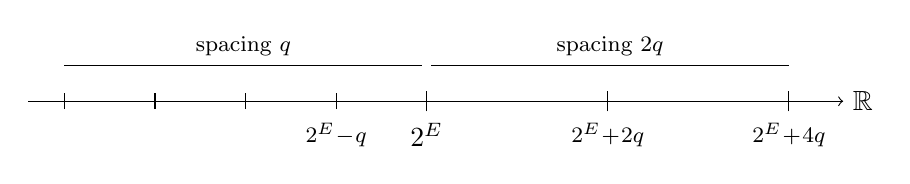
\begin{tikzpicture}[x=1.15cm,y=1cm]
  \draw[->] (-4.4,0) -- (4.6,0) node[right] {$\mathbb{R}$};
  \foreach \i in {-4,-3,-2,-1} \draw (\i,-0.1) -- (\i,0.1);
  \foreach \i in {0,2,4} \draw (\i,-0.13) -- (\i,0.13);
  \node[below] at (0,-0.15) {$2^E$};
  \node[below] at (-1,-0.15) {\footnotesize $2^E\!-\!q$};
  \node[below] at (2,-0.15) {\footnotesize $2^E\!+\!2q$};
  \node[below] at (4,-0.15) {\footnotesize $2^E\!+\!4q$};
  \draw (-4,0.45) -- (-0.05,0.45) node[midway,above] {\footnotesize spacing $q$};
  \draw (0.05,0.45) -- (4,0.45) node[midway,above] {\footnotesize spacing $2q$};
\end{tikzpicture}
\caption{The binary32 grid around $2^E$. The grid is finer below it, which is why a
result near $2^E$ gets less room.}
\end{figure}

\begin{lemma}[\lean{accept\_pos}, \lean{accept}]\label{lem:accept}
If $2^E \le |t|$ and $|Y - t| < \tfrac32 q$, then $\RN_{32}(Y)$ and $\RN_{32}(t)$ are
within one ulp.
\end{lemma}

\begin{lemma}[\lean{accept\_inner}, \lean{accept\_inner\_ge}]\label{lem:inner}
If $2^E + 2q \le |t|$ and $|Y - t| < 2q$, then $\RN_{32}(Y)$ and $\RN_{32}(t)$ are
within one ulp.
\end{lemma}

\begin{proof}[Proof of Lemma~\ref{lem:accept}]
Negating $t$, $Y$ and both results changes nothing, so take $t > 0$. A higher binade only
has a larger $q$, so take $2^E \le t < 2^{E+1}$. (\lean{accept} also requires
$-100 \le E$ and $|t| < 2^{100}$, which keep every value here in binary32's normal
range.) Let $a = \RN_{32}(t)$ and $y = \RN_{32}(Y)$. Three facts do the work:
\begin{enumerate}
\item rounding keeps order against any binary32 $F$: if $F \le X$ then
$F \le \RN_{32}(X)$, and likewise for $\ge$;
\item every binary32 at or above $2^E$ is a multiple of $2q$, and every multiple of $2q$
in $[2^E, 2^{E+1}]$ is a binary32, so any $X$ in that range rounds to within $q$ of itself;
\item the binary32 values in $[2^{E-1}, 2^E)$ are the multiples of $q$, so the two below
$2^E$ are $2^E - q$ and $2^E - 2q$.
\end{enumerate}
By (1) and (2), $2^E \le a \le 2^{E+1}$, $a$ is a multiple of $2q$, and $|a - t| \le q$.

\emph{Case $Y \ge 2^E$.} By (1), $y \ge 2^E$, so $y$ is a multiple of $2q$ too. If
$Y \le 2^{E+1}$, then $|y - Y| \le q$ by (2). If $Y > 2^{E+1}$, the binary32 $2^{E+1}$ lies
between $t$ and $Y$, so $|y - Y| \le Y - 2^{E+1} < Y - t < \tfrac32 q$. Either way,
\[
  |y - a| \le |y - Y| + |Y - t| + |t - a| < \tfrac32 q + \tfrac32 q + q = 4q .
\]
Two multiples of $2q$ less than $4q$ apart are equal or neighbours, and any binary32
between them would also be a multiple of $2q$, so there is none.

\emph{Case $Y < 2^E$.} Now $y$ can land on the finer grid. From the hypotheses,
$2^E - \tfrac32 q < Y$ and $t < 2^E + \tfrac32 q$. By (1), $y \le 2^E$. If
$Y \ge 2^E - q$, then (1) gives $y \ge 2^E - q$. Otherwise $Y$ is within $\tfrac12 q$ of
$2^E - q$ and further than that from $2^E - 2q$ and everything below it. So
$y \in \{2^E - q,\ 2^E\}$. Also $a \le t + q < 2^E + \tfrac52 q$, and $a$ is a multiple of
$2q$, so $a \in \{2^E,\ 2^E + 2q\}$.

If $a = 2^E$, then $y$ equals it or is its neighbour below. If $a = 2^E + 2q$, then $a$ is
at least as near to $t$ as $2^E$ is, so $t \ge 2^E + q$. Then $Y > t - \tfrac32 q \ge
2^E - \tfrac12 q$, which is nearer to $2^E$ than to $2^E - q$, so $y = 2^E$, the neighbour
below $a$.
\end{proof}

The constant cannot be raised. At $t = 2^E$, the value $Y = 2^E - \tfrac32 q$ is a tie that
round-to-even sends to $2^E - 2q$, leaving $2^E - q$ between it and $a = 2^E$. That is the
price of the finer grid, and Lemma~\ref{lem:inner} avoids it by keeping $t$ away from $2^E$.

Lemma~\ref{lem:inner} needs its margin only at the bottom of the binade: crossing the
top lands on a coarser grid, where $y$ can only be $2^{E+1}$, and in any higher binade
$\tfrac32 q'$ already exceeds $2q$.

\section{The kernel's error}\label{sec:error}

Let $r^* = m c - 1$, the exact value of $r$. Since $\log m = \log(mc) - \log c$,
\[
  Y - \log x = \bigl[P(r^*) - \log(1 + r^*)\bigr] + \text{rounding}.
\]
The polynomial's own error at $r^*$ is the only term that depends on the drift of $c$.

\begin{lemma}[\lean{kernel\_error}]\label{lem:error}
Let $|k| \le K \le 150$, $1 \le m \le 2$, $\tfrac{9}{20} \le c \le \tfrac{11}{10}$ and
$|mc - 1| \le \tfrac1{16}$. Then
\[
  |Y - (k \log 2 + \log m)| \le |P(r^*) - \log(1 + r^*)|
    + (10 + 3K)u + 16\eta + K|\mathtt{ln2} - \log 2|.
\]
\end{lemma}

\begin{proof}
Each instruction's rounding is bounded through the size of its argument, all of which are
below $110$. Writing each rounded value as its exact argument plus an error, $Y - \log x$
is a sum of: the term above; $P(r) - P(r^*)$, at most $\tfrac{11}{10}|r - r^*|$ with
$|r - r^*| \le 3u$; $k(\mathtt{ln2} - \log 2)$; the roundings of the log entry, $y_0$, $s$
and $Y$; and those of the polynomial's evaluation, which are scaled by $r^2$ and so are
tiny. The total of the coefficients is below the stated one.
\end{proof}

\begin{lemma}[\lean{ln2d\_err}]
$|\mathtt{ln2} - \log 2| \le 2^{-54}$, from
$\log 2 = \sum_{i \ge 1} 2^{-i}/i$ with 58 terms and Mathlib's bound on the rest.
\end{lemma}

\section{The polynomial's error}\label{sec:poly}

Let $e(r) = P(r) - \log(1 + r)$. Mathlib's
\lean{Real.abs\_log\_sub\_add\_sum\_range\_le} splits it into a polynomial and a remainder:
\[
  |e(r)| \le |Q(r)| + \frac{|r|^{10}}{1 - |r|},
  \qquad Q(r) = P(r) - \sum_{j=1}^{9} \frac{(-1)^{j+1} r^j}{j}.
\]
The $r$ term cancels, and $Q$ turns only at $r = 0$ and near
$-0.02023$, $-0.00135$ and $0.01839$ on $[-\tfrac1{16}, \tfrac1{16}]$.

\begin{lemma}[\lean{stretch1}\ldots\lean{stretch5}]
$Q$ is monotone on each of the five stretches between $\pm\tfrac1{16}$, $0$ and boxes of
half-width $2^{-20}$ around those three points.
\end{lemma}

\begin{proof}
The sign of $Q'$ on each stretch, by interval arithmetic with rational ends (a verified
Horner's rule, \lean{hornerIv}), bisecting where an interval is too wide. The check runs
in Lean's kernel.
\end{proof}

So over any range, the worst $|Q|$ is at the range's ends, clipped to each stretch, or
inside a box, where interval arithmetic bounds it (\lean{esup}). This is an exact
evaluation at points, so it loses nothing to a sampling resolution. The bound
$\mathtt{errSup}(\ell,h)$ is $\mathtt{esup}(\ell,h)$ plus the remainder's bound
$\rho^{10}/(1-\rho)$, where $\rho = \max(|\ell|, |h|)$.

\begin{theorem}[\lean{err\_sound}]
For $[\ell, h] \subseteq [-\tfrac1{16}, \tfrac1{16}]$ and $r \in [\ell, h]$,
$|e(r)| \le \mathtt{errSup}(\ell, h)$.
\end{theorem}

\section{One cell}\label{sec:cell}

For a box of significands $[m_a, m_b]$ and a window $[c_\ell, c_h]$, $r^*$ lies in
$[m_a c_\ell - 1,\ m_b c_h - 1]$. The check compares $\mathtt{errSup}$ of that range with
what acceptance allows, for three cases of the exponent:

\begin{center}
\begin{tabular}{lll}
\toprule
Case & Size of $t$ from below & Allowed error \\
\midrule
$k = 0$ & $\log m_a$ & \lean{tau} of that bound, minus rounding at $K = 0$ \\
$k = -1$ & $\log 2 - \log m_b$ & \lean{tau} of that bound, minus rounding at $K = 1$ \\
any other & $\tfrac12$ & $\tfrac32 2^{-25}$, minus rounding at $K = 150$ \\
\bottomrule
\end{tabular}
\end{center}

Here \lean{tau} takes $E$, the binade of the lower bound, and gives $2q$ when
Lemma~\ref{lem:inner} applies, $\tfrac32 q$ when the bound reaches $2^E$ but not $2^E + 2q$,
and $0$ when it is below $2^E$. The first two cases split the box in half on failure, to a
depth of 24, since a cell can straddle a binade of $t$. Lower bounds on the logs
come from the same series, summed exactly.

\begin{theorem}[\lean{side\_sound}]
If \lean{sideOK} returns \lean{true} for a cell and window, the conclusion of
Theorem~\ref{thm:main} holds for that window.
\end{theorem}

\lean{cells\_checked} then runs the check on all 512 sides in Lean's kernel, by
\lean{decide +kernel}, which adds no axioms. The windows themselves come from a search
(\lean{gen/Search.lean}) that is not trusted: it only proposes them.

\section{What limits the bound}\label{sec:limits}

Away from $x = 1$ the polynomial's error near the end of its range grows like $r^5/5$, and
the budget is one spacing of the smallest result in the cell. That result's binade sets the
steps in the bound: each halving of the budget shrinks the allowed $r$ by about
$2^{-1/5} \approx 0.87$.

Five sides stay well under the measured bound: cell 0 both ways, cell 1 downward, and
cell 255 both ways. All touch $x = 1$, where the budget is smallest. Two costs are likely
there, which we have not separated: the proof assumes an input may sit at its worst
rounding position, and those stretches hold few inputs, which may simply not include one;
and the rounding term weighs most there, because $c$ is not assumed to make $r$ exact.

\section{Toward the exact proof}\label{sec:exact}

The bound above treats all of a cell's inputs alike. Replacing the per-cell threshold with
each input's own slack, the distance from $\log x$ to the edge of its one-ulp region, would
clear almost every input at once for all $c$. The few left, near the edge, form a residue to
check at every $c$, either in Lean by an exact evaluator of the instructions or with the
existing scan as a certificate. That is future work.

\section*{Scope}

This proves \texttt{logf} only. \texttt{log2f} has the same structure; \texttt{log10f} and
\texttt{log1pf} add rounding tests and slow paths. FRECPE's table is taken from Arm's
pseudocode and matched against the hardware, not proved. The result concerns the instruction
sequence in Section~\ref{sec:model}.

\appendix
\section{The windows}\label{app:table}

Drifts in percent. ``Proven'' is $\varepsilon^\pm_i$ from Theorem~\ref{thm:main}; ``measured''
is B4's last passing drift over every input, on a 29-bit grid, which stops within a factor
$1 + 3/256$ of the first failure, so a proven value may lie slightly above it.

\begin{small}
\begin{longtable}{rlrrrr}
\toprule
Cell & $\hat c$ & Down, proven & Down, measured & Up, proven & Up, measured \\
\midrule
\endhead
\bottomrule
\endlastfoot
% Generated by gen/check.py.
0 & \texttt{0x1.ffp-1} & 0.0159 & 0.0252 & 0.0148 & 0.0224 \\
1 & \texttt{0x1.fdp-1} & 1.2539 & 2.5160 & 1.5550 & 1.5800 \\
2 & \texttt{0x1.fbp-1} & 2.6034 & 2.5990 & 2.5909 & 2.5710 \\
3 & \texttt{0x1.f9p-1} & 2.7384 & 2.7150 & 2.6010 & 2.5990 \\
4 & \texttt{0x1.f7p-1} & 2.7272 & 2.7150 & 2.8263 & 2.8040 \\
5 & \texttt{0x1.f5p-1} & 2.9161 & 2.8970 & 2.8427 & 2.8350 \\
6 & \texttt{0x1.f3p-1} & 2.8991 & 2.8970 & 2.8623 & 2.8350 \\
7 & \texttt{0x1.f1p-1} & 2.8790 & 2.8660 & 2.8850 & 2.8660 \\
8 & \texttt{0x1.fp-1} & 3.0518 & 3.0250 & 2.9820 & 2.9600 \\
9 & \texttt{0x1.eep-1} & 3.2956 & 3.2630 & 3.0102 & 2.9930 \\
10 & \texttt{0x1.ecp-1} & 3.2676 & 3.2630 & 3.0416 & 3.0250 \\
11 & \texttt{0x1.eap-1} & 3.2365 & 3.2280 & 3.0761 & 3.0580 \\
12 & \texttt{0x1.e8p-1} & 3.2025 & 3.1930 & 3.1138 & 3.0910 \\
13 & \texttt{0x1.e6p-1} & 3.1654 & 3.1590 & 3.1546 & 3.1250 \\
14 & \texttt{0x1.e5p-1} & 3.3252 & 3.2990 & 2.9859 & 2.9600 \\
15 & \texttt{0x1.e3p-1} & 3.2831 & 3.2630 & 3.0321 & 3.0250 \\
16 & \texttt{0x1.e1p-1} & 3.2380 & 3.2280 & 3.2667 & 3.2630 \\
17 & \texttt{0x1.dfp-1} & 3.5301 & 3.5200 & 3.4850 & 3.4820 \\
18 & \texttt{0x1.ddp-1} & 3.4791 & 3.4820 & 3.5411 & 3.5200 \\
19 & \texttt{0x1.dcp-1} & 3.6281 & 3.5970 & 3.3826 & 3.3710 \\
20 & \texttt{0x1.dap-1} & 3.5721 & 3.5590 & 3.4441 & 3.4450 \\
21 & \texttt{0x1.d8p-1} & 3.5131 & 3.4820 & 3.5087 & 3.4820 \\
22 & \texttt{0x1.d7p-1} & 3.6561 & 3.6370 & 3.3567 & 3.3350 \\
23 & \texttt{0x1.d5p-1} & 3.5920 & 3.5590 & 3.4267 & 3.4080 \\
24 & \texttt{0x1.d3p-1} & 3.5249 & 3.5200 & 3.5000 & 3.4820 \\
25 & \texttt{0x1.d2p-1} & 3.6619 & 3.6370 & 3.3543 & 3.3350 \\
26 & \texttt{0x1.dp-1} & 3.5898 & 3.5590 & 3.4330 & 3.4080 \\
27 & \texttt{0x1.cep-1} & 3.5146 & 3.4820 & 3.5150 & 3.4820 \\
28 & \texttt{0x1.cdp-1} & 3.6458 & 3.6370 & 3.3756 & 3.3710 \\
29 & \texttt{0x1.cbp-1} & 3.5655 & 3.5590 & 3.4630 & 3.4450 \\
30 & \texttt{0x1.c9p-1} & 3.4821 & 3.4820 & 3.5537 & 3.5200 \\
31 & \texttt{0x1.c8p-1} & 3.6075 & 3.5970 & 3.4204 & 3.4080 \\
32 & \texttt{0x1.c6p-1} & 3.5190 & 3.5200 & 3.5166 & 3.4820 \\
33 & \texttt{0x1.c5p-1} & 3.6406 & 3.6370 & 3.3874 & 3.3710 \\
34 & \texttt{0x1.c3p-1} & 3.5470 & 3.5200 & 3.8150 & 3.7980 \\
35 & \texttt{0x1.c2p-1} & 4.0802 & 4.0530 & 3.7915 & 3.7570 \\
36 & \texttt{0x1.cp-1} & 3.9820 & 3.9660 & 3.8991 & 3.8810 \\
37 & \texttt{0x1.bfp-1} & 4.0956 & 4.0970 & 3.7773 & 3.7570 \\
38 & \texttt{0x1.bdp-1} & 3.9922 & 3.9660 & 3.8904 & 3.8810 \\
39 & \texttt{0x1.bcp-1} & 4.1022 & 4.0970 & 3.7726 & 3.7570 \\
40 & \texttt{0x1.bap-1} & 3.9937 & 3.9660 & 3.8912 & 3.8810 \\
41 & \texttt{0x1.b9p-1} & 4.1000 & 4.0970 & 3.7773 & 3.7570 \\
42 & \texttt{0x1.b7p-1} & 3.9864 & 3.9660 & 3.9015 & 3.8810 \\
43 & \texttt{0x1.b6p-1} & 4.0890 & 4.0530 & 3.7915 & 3.7570 \\
44 & \texttt{0x1.b4p-1} & 3.9702 & 3.9660 & 3.9212 & 3.8810 \\
45 & \texttt{0x1.b3p-1} & 4.0692 & 4.0530 & 3.8152 & 3.7980 \\
46 & \texttt{0x1.b1p-1} & 3.9453 & 3.9230 & 3.9505 & 3.9230 \\
47 & \texttt{0x1.bp-1} & 4.0406 & 4.0090 & 3.8484 & 3.8390 \\
48 & \texttt{0x1.aep-1} & 3.9114 & 3.8810 & 3.9894 & 3.9660 \\
49 & \texttt{0x1.adp-1} & 4.0032 & 3.9660 & 3.8912 & 3.8810 \\
50 & \texttt{0x1.acp-1} & 4.0934 & 4.0530 & 3.7947 & 3.7980 \\
51 & \texttt{0x1.aap-1} & 3.9570 & 3.9230 & 3.9434 & 3.9230 \\
52 & \texttt{0x1.a9p-1} & 4.0436 & 4.0090 & 3.8508 & 3.8390 \\
53 & \texttt{0x1.a7p-1} & 3.9019 & 3.8810 & 4.0052 & 4.0090 \\
54 & \texttt{0x1.a6p-1} & 3.9849 & 3.9660 & 3.9165 & 3.8810 \\
55 & \texttt{0x1.a5p-1} & 4.0663 & 4.0530 & 3.8295 & 3.7980 \\
56 & \texttt{0x1.a3p-1} & 3.9173 & 3.8810 & 3.9918 & 3.9660 \\
57 & \texttt{0x1.a2p-1} & 3.9952 & 3.9660 & 3.9086 & 3.8810 \\
58 & \texttt{0x1.a1p-1} & 4.0714 & 4.0530 & 3.8271 & 3.7980 \\
59 & \texttt{0x1.9fp-1} & 3.9151 & 3.8810 & 3.9973 & 3.9660 \\
60 & \texttt{0x1.9ep-1} & 3.9878 & 3.9660 & 3.9196 & 3.8810 \\
61 & \texttt{0x1.9dp-1} & 4.0590 & 4.0530 & 3.8437 & 3.8390 \\
62 & \texttt{0x1.9cp-1} & 4.1285 & 4.0970 & 3.7694 & 3.7570 \\
63 & \texttt{0x1.9ap-1} & 3.9629 & 3.9660 & 3.9498 & 3.9230 \\
64 & \texttt{0x1.99p-1} & 4.0289 & 4.0090 & 3.8793 & 3.8810 \\
65 & \texttt{0x1.98p-1} & 4.0934 & 4.0530 & 3.8105 & 3.7980 \\
66 & \texttt{0x1.96p-1} & 3.9203 & 3.8810 & 3.9989 & 3.9660 \\
67 & \texttt{0x1.95p-1} & 3.9812 & 3.9660 & 3.9339 & 3.9230 \\
68 & \texttt{0x1.94p-1} & 4.0406 & 4.0090 & 3.8706 & 3.8390 \\
69 & \texttt{0x1.93p-1} & 4.0985 & 4.0970 & 3.8089 & 3.7980 \\
70 & \texttt{0x1.91p-1} & 3.9159 & 3.8810 & 4.0076 & 4.0090 \\
71 & \texttt{0x1.9p-1} & 3.9702 & 3.9660 & 3.9498 & 3.9230 \\
72 & \texttt{0x1.8fp-1} & 4.0231 & 4.0090 & 3.9850 & 3.9660 \\
73 & \texttt{0x1.8ep-1} & 4.5714 & 4.5650 & 4.3514 & 4.3250 \\
74 & \texttt{0x1.8dp-1} & 4.6210 & 4.6150 & 4.2982 & 4.2780 \\
75 & \texttt{0x1.8bp-1} & 4.4276 & 4.4190 & 4.5105 & 4.4680 \\
76 & \texttt{0x1.8ap-1} & 4.4737 & 4.4680 & 4.4611 & 4.4190 \\
77 & \texttt{0x1.89p-1} & 4.5182 & 4.5160 & 4.4134 & 4.3720 \\
78 & \texttt{0x1.88p-1} & 4.5612 & 4.5160 & 4.3673 & 4.3250 \\
79 & \texttt{0x1.87p-1} & 4.6028 & 4.5650 & 4.3228 & 4.3250 \\
80 & \texttt{0x1.86p-1} & 4.6428 & 4.6150 & 4.2799 & 4.2780 \\
81 & \texttt{0x1.84p-1} & 4.4357 & 4.4190 & 4.5074 & 4.4680 \\
82 & \texttt{0x1.83p-1} & 4.4722 & 4.4680 & 4.4683 & 4.4680 \\
83 & \texttt{0x1.82p-1} & 4.5073 & 4.4680 & 4.4309 & 4.4190 \\
84 & \texttt{0x1.81p-1} & 4.5408 & 4.5160 & 4.3951 & 4.3720 \\
85 & \texttt{0x1.8p-1} & 4.5729 & 4.5650 & 4.3609 & 4.3250 \\
86 & \texttt{0x1.7fp-1} & 4.6035 & 4.5650 & 4.3283 & 4.3250 \\
87 & \texttt{0x1.7ep-1} & 4.6326 & 4.6150 & 4.2974 & 4.2780 \\
88 & \texttt{0x1.7cp-1} & 4.4094 & 4.3720 & 4.5424 & 4.5160 \\
89 & \texttt{0x1.7bp-1} & 4.4349 & 4.4190 & 4.5153 & 4.5160 \\
90 & \texttt{0x1.7ap-1} & 4.4591 & 4.4190 & 4.4898 & 4.4680 \\
91 & \texttt{0x1.79p-1} & 4.4817 & 4.4680 & 4.4659 & 4.4680 \\
92 & \texttt{0x1.78p-1} & 4.5029 & 4.4680 & 4.4436 & 4.4190 \\
93 & \texttt{0x1.77p-1} & 4.5226 & 4.5160 & 4.4230 & 4.4190 \\
94 & \texttt{0x1.76p-1} & 4.5408 & 4.5160 & 4.4039 & 4.3720 \\
95 & \texttt{0x1.75p-1} & 4.5576 & 4.5160 & 4.3864 & 4.3720 \\
96 & \texttt{0x1.74p-1} & 4.5729 & 4.5650 & 4.3705 & 4.3720 \\
97 & \texttt{0x1.73p-1} & 4.5867 & 4.5650 & 4.3561 & 4.3250 \\
98 & \texttt{0x1.72p-1} & 4.5991 & 4.5650 & 4.3434 & 4.3250 \\
99 & \texttt{0x1.71p-1} & 4.6100 & 4.5650 & 4.3323 & 4.3250 \\
100 & \texttt{0x1.7p-1} & 4.6195 & 4.6150 & 4.3228 & 4.2780 \\
101 & \texttt{0x1.6fp-1} & 4.6275 & 4.6150 & 4.3149 & 4.2780 \\
102 & \texttt{0x1.6ep-1} & 4.6341 & 4.6150 & 4.3085 & 4.2780 \\
103 & \texttt{0x1.6dp-1} & 4.6391 & 4.6150 & 4.3037 & 4.2780 \\
104 & \texttt{0x1.6cp-1} & 4.6428 & 4.6150 & 4.3006 & 4.2780 \\
105 & \texttt{0x1.6bp-1} & 4.6450 & 4.6150 & 4.2990 & 4.2780 \\
106 & \texttt{0x1.6ap-1} & 4.6457 & 4.6150 & 4.2990 & 4.2780 \\
107 & \texttt{0x1.69p-1} & 4.6450 & 4.6150 & 4.3006 & 4.2780 \\
108 & \texttt{0x1.68p-1} & 4.6428 & 4.6150 & 4.3037 & 4.2780 \\
109 & \texttt{0x1.67p-1} & 4.6391 & 4.6150 & 4.3085 & 4.2780 \\
110 & \texttt{0x1.66p-1} & 4.6341 & 4.6150 & 4.3149 & 4.2780 \\
111 & \texttt{0x1.65p-1} & 4.6275 & 4.6150 & 4.3228 & 4.3250 \\
112 & \texttt{0x1.64p-1} & 4.6195 & 4.6150 & 4.3323 & 4.3250 \\
113 & \texttt{0x1.63p-1} & 4.6100 & 4.5650 & 4.3434 & 4.3250 \\
114 & \texttt{0x1.62p-1} & 4.5991 & 4.5650 & 4.3561 & 4.3250 \\
115 & \texttt{0x1.61p-1} & 4.5867 & 4.5650 & 4.3705 & 4.3720 \\
116 & \texttt{0x1.6p-1} & 4.5729 & 4.5650 & 4.3864 & 4.3720 \\
117 & \texttt{0x1.5fp-1} & 4.5576 & 4.5160 & 4.4039 & 4.3720 \\
118 & \texttt{0x1.5ep-1} & 4.5408 & 4.5160 & 4.4230 & 4.4190 \\
119 & \texttt{0x1.5dp-1} & 4.5226 & 4.5160 & 4.4436 & 4.4190 \\
120 & \texttt{0x1.5cp-1} & 4.5029 & 4.4680 & 4.4659 & 4.4680 \\
121 & \texttt{0x1.5bp-1} & 4.4817 & 4.4680 & 4.4898 & 4.4680 \\
122 & \texttt{0x1.5ap-1} & 4.4591 & 4.4190 & 4.5153 & 4.5160 \\
123 & \texttt{0x1.59p-1} & 4.4349 & 4.4190 & 4.5424 & 4.5160 \\
124 & \texttt{0x1.58p-1} & 4.4094 & 4.3720 & 4.5711 & 4.5650 \\
125 & \texttt{0x1.58p-1} & 4.6602 & 4.6150 & 4.2974 & 4.2780 \\
126 & \texttt{0x1.57p-1} & 4.6326 & 4.6150 & 4.3283 & 4.3250 \\
127 & \texttt{0x1.56p-1} & 4.6035 & 4.5650 & 4.3609 & 4.3720 \\
128 & \texttt{0x1.55p-1} & 4.5729 & 4.5650 & 4.3951 & 4.3720 \\
129 & \texttt{0x1.54p-1} & 4.5408 & 4.5160 & 4.4309 & 4.4190 \\
130 & \texttt{0x1.53p-1} & 4.5073 & 4.4680 & 4.4683 & 4.4680 \\
131 & \texttt{0x1.52p-1} & 4.4722 & 4.4680 & 4.5074 & 4.4680 \\
132 & \texttt{0x1.51p-1} & 4.4357 & 4.4190 & 4.5480 & 4.5160 \\
133 & \texttt{0x1.51p-1} & 4.6813 & 4.6650 & 4.2799 & 4.2780 \\
134 & \texttt{0x1.5p-1} & 4.6428 & 4.6150 & 4.3228 & 4.3250 \\
135 & \texttt{0x1.4fp-1} & 4.6028 & 4.5650 & 4.3673 & 4.3250 \\
136 & \texttt{0x1.4ep-1} & 4.5612 & 4.5160 & 4.4134 & 4.3720 \\
137 & \texttt{0x1.4dp-1} & 4.5182 & 4.5160 & 4.4611 & 4.4190 \\
138 & \texttt{0x1.4cp-1} & 4.4737 & 4.4680 & 4.5105 & 4.4680 \\
139 & \texttt{0x1.4bp-1} & 4.4276 & 4.4190 & 4.5616 & 4.5160 \\
140 & \texttt{0x1.4bp-1} & 4.6690 & 4.6650 & 4.2982 & 4.2780 \\
141 & \texttt{0x1.4ap-1} & 4.6210 & 4.6150 & 4.3514 & 4.3250 \\
142 & \texttt{0x1.49p-1} & 4.2538 & 4.2320 & 3.8935 & 3.8810 \\
143 & \texttt{0x1.48p-1} & 4.0231 & 4.0090 & 3.9498 & 3.9230 \\
144 & \texttt{0x1.47p-1} & 3.9702 & 3.9660 & 4.0076 & 3.9660 \\
145 & \texttt{0x1.46p-1} & 3.9159 & 3.8810 & 4.0671 & 4.0530 \\
146 & \texttt{0x1.46p-1} & 4.1549 & 4.1410 & 3.8089 & 3.7980 \\
147 & \texttt{0x1.45p-1} & 4.0985 & 4.0970 & 3.8706 & 3.8390 \\
148 & \texttt{0x1.44p-1} & 4.0406 & 4.0090 & 3.9339 & 3.9230 \\
149 & \texttt{0x1.43p-1} & 3.9812 & 3.9660 & 3.9989 & 3.9660 \\
150 & \texttt{0x1.42p-1} & 3.9203 & 3.9230 & 4.0656 & 4.0530 \\
151 & \texttt{0x1.42p-1} & 4.1563 & 4.1410 & 3.8105 & 3.7980 \\
152 & \texttt{0x1.41p-1} & 4.0934 & 4.0530 & 3.8793 & 3.8390 \\
153 & \texttt{0x1.4p-1} & 4.0289 & 4.0090 & 3.9498 & 3.9230 \\
154 & \texttt{0x1.3fp-1} & 3.9629 & 3.9230 & 4.0219 & 4.0090 \\
155 & \texttt{0x1.3fp-1} & 4.1965 & 4.1860 & 3.7694 & 3.7570 \\
156 & \texttt{0x1.3ep-1} & 4.1285 & 4.0970 & 3.8437 & 3.8390 \\
157 & \texttt{0x1.3dp-1} & 4.0590 & 4.0530 & 3.9196 & 3.8810 \\
158 & \texttt{0x1.3cp-1} & 3.9878 & 3.9660 & 3.9973 & 3.9660 \\
159 & \texttt{0x1.3bp-1} & 3.9151 & 3.8810 & 4.0767 & 4.0530 \\
160 & \texttt{0x1.3bp-1} & 4.1461 & 4.1410 & 3.8271 & 3.7980 \\
161 & \texttt{0x1.3ap-1} & 4.0714 & 4.0530 & 3.9086 & 3.8810 \\
162 & \texttt{0x1.39p-1} & 3.9952 & 3.9660 & 3.9918 & 3.9660 \\
163 & \texttt{0x1.38p-1} & 3.9173 & 3.8810 & 4.0767 & 4.0530 \\
164 & \texttt{0x1.38p-1} & 4.1461 & 4.1410 & 3.8295 & 3.7980 \\
165 & \texttt{0x1.37p-1} & 4.0663 & 4.0530 & 3.9165 & 3.8810 \\
166 & \texttt{0x1.36p-1} & 3.9849 & 3.9660 & 4.0052 & 3.9660 \\
167 & \texttt{0x1.35p-1} & 3.9019 & 3.8810 & 4.0957 & 4.0970 \\
168 & \texttt{0x1.35p-1} & 4.1285 & 4.0970 & 3.8508 & 3.8390 \\
169 & \texttt{0x1.34p-1} & 4.0436 & 4.0090 & 3.9434 & 3.9230 \\
170 & \texttt{0x1.33p-1} & 3.9570 & 3.9230 & 4.0378 & 4.0090 \\
171 & \texttt{0x1.33p-1} & 4.1819 & 4.1410 & 3.7947 & 3.7570 \\
172 & \texttt{0x1.32p-1} & 4.0934 & 4.0530 & 3.8912 & 3.8810 \\
173 & \texttt{0x1.31p-1} & 4.0032 & 3.9660 & 3.9894 & 3.9660 \\
174 & \texttt{0x1.3p-1} & 3.9114 & 3.8810 & 4.0894 & 4.0530 \\
175 & \texttt{0x1.3p-1} & 4.1344 & 4.0970 & 3.8484 & 3.8390 \\
176 & \texttt{0x1.2fp-1} & 4.0406 & 4.0090 & 3.9505 & 3.9230 \\
177 & \texttt{0x1.2ep-1} & 3.9453 & 3.9230 & 4.0545 & 4.0530 \\
178 & \texttt{0x1.2ep-1} & 4.1666 & 4.1410 & 3.8152 & 3.7980 \\
179 & \texttt{0x1.2dp-1} & 4.0692 & 4.0530 & 3.9212 & 3.9230 \\
180 & \texttt{0x1.2cp-1} & 3.9702 & 3.9660 & 4.0290 & 4.0090 \\
181 & \texttt{0x1.2cp-1} & 4.1900 & 4.1860 & 3.7915 & 3.7570 \\
182 & \texttt{0x1.2bp-1} & 4.0890 & 4.0530 & 3.9014 & 3.8810 \\
183 & \texttt{0x1.2ap-1} & 3.9864 & 3.9660 & 4.0132 & 4.0090 \\
184 & \texttt{0x1.2ap-1} & 4.2046 & 4.1860 & 3.7773 & 3.7570 \\
185 & \texttt{0x1.29p-1} & 4.1000 & 4.0970 & 3.8912 & 3.8810 \\
186 & \texttt{0x1.28p-1} & 3.9937 & 3.9660 & 4.0068 & 4.0090 \\
187 & \texttt{0x1.28p-1} & 4.2104 & 4.1860 & 3.7726 & 3.7570 \\
188 & \texttt{0x1.27p-1} & 4.1022 & 4.0970 & 3.8904 & 3.8810 \\
189 & \texttt{0x1.26p-1} & 3.9922 & 3.9660 & 4.0100 & 4.0090 \\
190 & \texttt{0x1.26p-1} & 4.2075 & 4.1860 & 3.7773 & 3.7570 \\
191 & \texttt{0x1.25p-1} & 4.0956 & 4.0970 & 3.8991 & 3.8810 \\
192 & \texttt{0x1.24p-1} & 3.9820 & 3.9660 & 4.0227 & 4.0090 \\
193 & \texttt{0x1.24p-1} & 4.1958 & 4.1860 & 3.7915 & 3.7570 \\
194 & \texttt{0x1.23p-1} & 4.0802 & 4.0530 & 3.9173 & 3.8810 \\
195 & \texttt{0x1.22p-1} & 3.7260 & 3.7160 & 3.6161 & 3.5970 \\
196 & \texttt{0x1.22p-1} & 3.7604 & 3.7570 & 3.3874 & 3.3710 \\
197 & \texttt{0x1.21p-1} & 3.6406 & 3.6370 & 3.5166 & 3.4820 \\
198 & \texttt{0x1.2p-1} & 3.5190 & 3.4820 & 3.6477 & 3.6370 \\
199 & \texttt{0x1.2p-1} & 3.7311 & 3.7160 & 3.4204 & 3.4080 \\
200 & \texttt{0x1.1fp-1} & 3.6075 & 3.5970 & 3.5537 & 3.5200 \\
201 & \texttt{0x1.1ep-1} & 3.4821 & 3.4820 & 3.6889 & 3.6760 \\
202 & \texttt{0x1.1ep-1} & 3.6928 & 3.6760 & 3.4630 & 3.4450 \\
203 & \texttt{0x1.1dp-1} & 3.5655 & 3.5590 & 3.6003 & 3.5970 \\
204 & \texttt{0x1.1dp-1} & 3.7751 & 3.7570 & 3.3756 & 3.3710 \\
205 & \texttt{0x1.1cp-1} & 3.6458 & 3.6370 & 3.5150 & 3.4820 \\
206 & \texttt{0x1.1bp-1} & 3.5146 & 3.4820 & 3.6564 & 3.6370 \\
207 & \texttt{0x1.1bp-1} & 3.7230 & 3.7160 & 3.4330 & 3.4080 \\
208 & \texttt{0x1.1ap-1} & 3.5898 & 3.5590 & 3.5766 & 3.5590 \\
209 & \texttt{0x1.1ap-1} & 3.7971 & 3.7980 & 3.3543 & 3.3350 \\
210 & \texttt{0x1.19p-1} & 3.6619 & 3.6370 & 3.5000 & 3.4820 \\
211 & \texttt{0x1.18p-1} & 3.5249 & 3.5200 & 3.6477 & 3.6370 \\
212 & \texttt{0x1.18p-1} & 3.7311 & 3.7160 & 3.4267 & 3.4080 \\
213 & \texttt{0x1.17p-1} & 3.5920 & 3.5590 & 3.5766 & 3.5590 \\
214 & \texttt{0x1.17p-1} & 3.7971 & 3.7980 & 3.3567 & 3.3350 \\
215 & \texttt{0x1.16p-1} & 3.6561 & 3.6370 & 3.5087 & 3.4820 \\
216 & \texttt{0x1.15p-1} & 3.5131 & 3.4820 & 3.6628 & 3.6370 \\
217 & \texttt{0x1.15p-1} & 3.7171 & 3.7160 & 3.4441 & 3.4450 \\
218 & \texttt{0x1.14p-1} & 3.5721 & 3.5590 & 3.6003 & 3.5970 \\
219 & \texttt{0x1.14p-1} & 3.7751 & 3.7570 & 3.3826 & 3.3710 \\
220 & \texttt{0x1.13p-1} & 3.6281 & 3.5970 & 3.5410 & 3.5200 \\
221 & \texttt{0x1.12p-1} & 3.4791 & 3.4450 & 3.7015 & 3.6760 \\
222 & \texttt{0x1.12p-1} & 3.6811 & 3.6760 & 3.4850 & 3.4820 \\
223 & \texttt{0x1.11p-1} & 3.5301 & 3.5200 & 3.6477 & 3.6370 \\
224 & \texttt{0x1.11p-1} & 3.5883 & 3.5590 & 3.0816 & 3.0580 \\
225 & \texttt{0x1.1p-1} & 3.2380 & 3.2280 & 3.2459 & 3.2280 \\
226 & \texttt{0x1.1p-1} & 3.4387 & 3.4080 & 3.0321 & 3.0250 \\
227 & \texttt{0x1.0fp-1} & 3.2831 & 3.2630 & 3.1986 & 3.1930 \\
228 & \texttt{0x1.0fp-1} & 3.4829 & 3.4820 & 2.9859 & 2.9600 \\
229 & \texttt{0x1.0ep-1} & 3.3252 & 3.2990 & 3.1546 & 3.1250 \\
230 & \texttt{0x1.0dp-1} & 3.1654 & 3.1590 & 3.3255 & 3.2990 \\
231 & \texttt{0x1.0dp-1} & 3.3643 & 3.3350 & 3.1137 & 3.0910 \\
232 & \texttt{0x1.0cp-1} & 3.2025 & 3.1930 & 3.2869 & 3.2630 \\
233 & \texttt{0x1.0cp-1} & 3.4004 & 3.3710 & 3.0761 & 3.0580 \\
234 & \texttt{0x1.0bp-1} & 3.2365 & 3.2280 & 3.2514 & 3.2280 \\
235 & \texttt{0x1.0bp-1} & 3.4336 & 3.4080 & 3.0415 & 3.0250 \\
236 & \texttt{0x1.0ap-1} & 3.2676 & 3.2630 & 3.2191 & 3.1930 \\
237 & \texttt{0x1.0ap-1} & 3.4638 & 3.4450 & 3.0102 & 2.9930 \\
238 & \texttt{0x1.09p-1} & 3.2956 & 3.2630 & 3.1900 & 3.1930 \\
239 & \texttt{0x1.09p-1} & 3.4910 & 3.4820 & 2.9819 & 2.9600 \\
240 & \texttt{0x1.08p-1} & 3.1002 & 3.0910 & 2.8850 & 2.8660 \\
241 & \texttt{0x1.07p-1} & 2.8790 & 2.8660 & 3.0688 & 3.0580 \\
242 & \texttt{0x1.07p-1} & 3.0740 & 3.0580 & 2.8623 & 2.8350 \\
243 & \texttt{0x1.06p-1} & 2.8991 & 2.8970 & 3.0484 & 3.0250 \\
244 & \texttt{0x1.06p-1} & 3.0933 & 3.0910 & 2.8427 & 2.8350 \\
245 & \texttt{0x1.05p-1} & 2.9161 & 2.8970 & 3.0311 & 3.0250 \\
246 & \texttt{0x1.05p-1} & 3.1095 & 3.0910 & 2.8262 & 2.8040 \\
247 & \texttt{0x1.04p-1} & 2.9302 & 2.9280 & 3.0169 & 2.9930 \\
248 & \texttt{0x1.04p-1} & 2.9322 & 2.9280 & 2.6010 & 2.5990 \\
249 & \texttt{0x1.03p-1} & 2.7384 & 2.7150 & 2.7936 & 2.7740 \\
250 & \texttt{0x1.03p-1} & 2.9306 & 2.9280 & 2.5908 & 2.5710 \\
251 & \texttt{0x1.02p-1} & 2.7465 & 2.7440 & 2.7858 & 2.7740 \\
252 & \texttt{0x1.02p-1} & 2.7981 & 2.7740 & 2.4327 & 2.4100 \\
253 & \texttt{0x1.01p-1} & 2.6086 & 2.5990 & 2.6296 & 2.6280 \\
254 & \texttt{0x1.01p-1} & 1.4483 & 1.4480 & 1.1583 & 1.1540 \\
255 & \texttt{0x1p-1} & 0.0125 & 0.0175 & 0.0118 & 0.0162 \\

\end{longtable}
\end{small}

\end{document}
